\section{Literature Review}
\label{sec:review}
%
Itemization
\begin{itemize}
\item Item 1.
\item Item 2.
\item \ldots

\end{itemize}

\begin{equation}
\dot{x}=Ax+Bu+B_dw
\end{equation}
%
 Refering a chapter in the main text. For instance Chapter~\ref{sec:review} 
%
\begin{eqnarray} \nonumber
E = 210000\Unit{\mathrm{\frac{N}{mm^2}}}
\end{eqnarray}
%

%
\begin{eqnarray}\nonumber
\rho = 7{,}85\Unit{\mathrm{\frac{g}{cm^3}}}=
7850\Unit{\mathrm{\frac{kg}{m^3}}}.
\end{eqnarray}
%

\begin{equation}
  \Delta \boldsymbol{r}_k= \boldsymbol{r}_{\mathrm{GBE}_k} -
  \boldsymbol{r}_{\mathrm{C}_k} = (x_{\mathrm{GBE}_k} - x_{\mathrm{C}_k},
  y_{\mathrm{GBE}_k} - y_{\mathrm{C}_k})^T = (\Delta x_k,\Delta
  y_k)^T
\end{equation}
%
 $k=2 \dots n$

%
\begin{equation}
  || \boldsymbol{r}_{\mathrm{GBE}_k} -
  \boldsymbol{r}_{\mathrm{C}_k} || \leq  r_{kj},
\end{equation}
%
 $k$  $j$ 
%

\begin{equation}\label{26}
    {\rm rank} \; \boldsymbol{Q}_{\rm B} = {\rm rank} \left[
    \begin{array}{c}
    \bs C \\
    \bs{CA} \\
    \bs{CA}^2 \\
    \vdots \\
    \bs{CA}^{n-1}
    \end{array} \right] = n.
\end{equation}
%

%
\begin{eqnarray}
K_\varphi & = & 3.64\;\mr{\frac{V}{rad}}\quad\mbox{and}\\
K_x & = & 28.32 \;\mr{\frac{V}{m}}.
\end{eqnarray}
%
%
\subsection{Name of a subsection}
\label{subsec:xxxxx}
%
 $q_1,q_2$ and
$q_3$ (see Fig.~\ref{fig:drei_arm}).
%
\subsection{Another subsection}


%\begin{figure}[!htb]
%  \begin{center}
%    \leavevmode
%    \psfrag{F_Last}[][]{\footnotesize{$F_\mathrm{Last}$}}
%    \psfrag{1}[][]{\footnotesize{P$_1$}}
%    \psfrag{2}[r][]{\footnotesize{Lisa$_2$}}
%    \psfrag{3}[][]{\footnotesize{P$_3$}}
%    \psfrag{4}[][]{\footnotesize{P$_4$}}
%    \psfrag{l,m}[][]{\footnotesize{$l, m$}}
%    \psfrag{q1}[][]{\footnotesize{$q_1$}}
%    \psfrag{-q2}[r][]{\footnotesize{$-q_2$}}
%    \psfrag{-q3}[][]{\footnotesize{$-q_3$}}
%    \psfrag{x0}[][]{\footnotesize{$x_0$}}
%    \psfrag{y0}[][]{\footnotesize{$y_0$}}
%    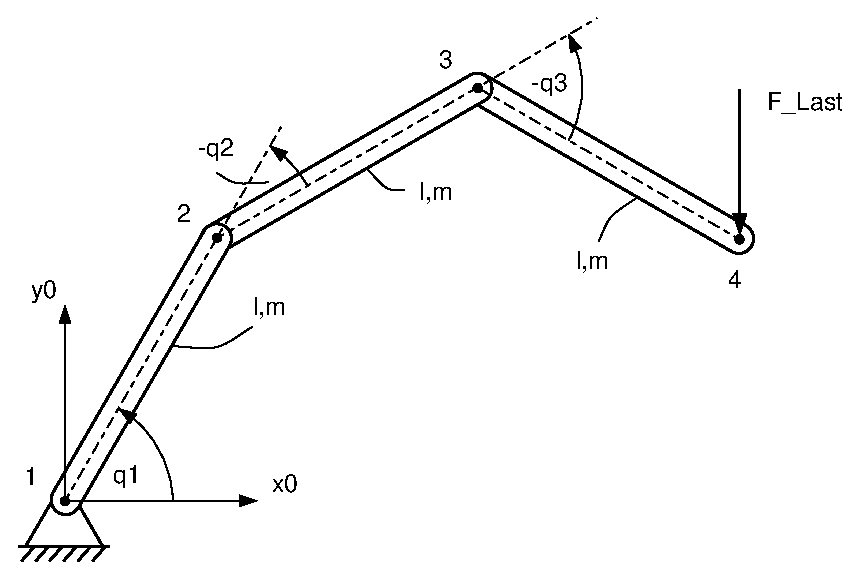
\includegraphics[width=0.64\textwidth]{Figures/drei_arm.eps}
%  \end{center}
%   \hangcaption[The caption for the figure (Add more)]{The caption for the figure should always be at the bottom of the figure\\ The caption can overflow to the next line\ldots}
%  \label{fig:drei_arm}
%\end{figure}



%
\begin{table}[!t]
  \begin{center}
    \leavevmode
    \caption[To appear in the list of tables]{Caption for the table should be at the top of the table\\It can also overflow to next line}   
     \begin{tabular}{rlc}\hline
      First column & Second column & Third column \\ \hline
      1 & 2 & 4\\
      4 & 6 & 23\\
      34 & 2 & 0 \\ \hline
    \end{tabular}
    \label{tab:zweiarmsystemtab}
  \end{center}
\end{table}
%
